\documentclass[number]{ximera}

%My github password is ximera1
%My GeoGebra password is Ximera1

%\usepackage{tikz}

\renewcommand{\theenumi}{\arabic{enumi}.}


% set font encoding for PDFLaTeX, XeLaTeX, or LuaTeX
\usepackage{ifxetex,ifluatex}
\newif\ifxetexorluatex
\ifxetex
  \xetexorluatextrue
\else
  \ifluatex
    \xetexorluatextrue
  \else
    \xetexorluatexfalse
  \fi
\fi

\ifxetexorluatex
  \usepackage{fontspec}
\else
  \usepackage[T1]{fontenc}
  \usepackage[utf8]{inputenc}
  \usepackage{lmodern}
\fi

\usepackage{hyperref}
\usepackage{tikz} %% Adding this here so it's not manually added elsewhere
\title{Angle Sum Formulas - Part I}
\author{Univ. of Minnesota MathCEP}


% Enable SageTeX to run SageMath code right inside this LaTeX file.
% http://mirrors.ctan.org/macros/latex/contrib/sagetex/sagetexpackage.pdf
% \usepackage{sagetex}

\begin{document}

\begin{abstract}
  In this activity, you will discover the issue involved in using the Law of Sines and Law of Cosines to solve triangles.
\end{abstract}

\maketitle

%7\begin{enumerate} 

\begin{enumerate}

\item Find the following distances:

\begin{enumerate}

\item Find the distance between $(4,0)$ and $(-2,0)$

\item Find the distance between $(4,3)$ and $(-2,3)$

\item Find the distance between $(4,3)$ and $(4,6)$

\item Find the distance between $(-2,3)$ and $(4,6)$

\item Find the distance between $(-2,3)$ and $(h,k)$

\item Find the distance between $(x,y)$ and $(h,k)$

\end{enumerate}

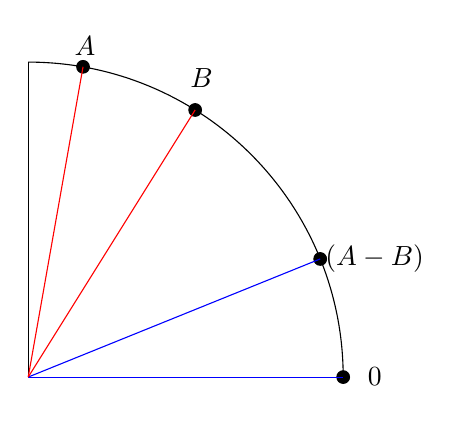
\begin{tikzpicture}[scale=4]

\draw (0,1) arc [radius=1, start angle=90, end angle=0];
\draw [fill] (1,0) circle [radius=0.02];
\draw [fill] (.927,.375) circle [radius=0.02];
\draw [fill] (.174,.985) circle [radius=0.02];
\draw [fill] (.530,.848) circle [radius=0.02];
\draw (0,0) -- (0,1);
\draw [blue] (0,0) -- (1,0);
\draw [blue] (0,0) -- (.927,.375);
\draw [red] (0,0) -- (.174,.985);
\draw [red] (0,0) -- (.530,.848);
\node at (.18,1.05) {$A$};
\node at (.55,.95) {$B$};
\node at (1.1,0.375) {$(A-B)$};
\node at (1.1,0) {$0$};
\end{tikzpicture}



\item Let $A$ and $B$ be first quadrant angles with $A > B > (A-B) > 0$. 

\begin{enumerate}

\item In the picture above, label the $x$- and $y$-coordinates of the points associated with $A$, $B$, $A-B$, and $0$.

(Hint: the ordered pair for the angle $0$ is $(1,0)$, from the unit circle. The others will involve $sin$ and $cos$.)

\item Find a formula for the distance between the points associated with angles $A$ and $B$.

\item Find a formula for the distance between the points associated with angles $(A-B)$ and $0$.

\item Explain why the distances found in part b) and part c) are the same.

\item Set the distances in part b) and part c) equal to each other and simplify. Your result should be a formula for $\cos(A-B)$.

\end{enumerate}

\item Let $C = -B$

\begin{enumerate}

\item Using your answer to 2e) write the formula for $\cos(A-C)$.

\item How does $\cos (C)$ relate to $\cos (B)$? How does $\sin (C)$ relate to $\sin (B)$? 

\item In 3a) replace $C$ with $-B$.

\item Using 3b), simplify the equation in 3c). Your result should be a formula for $\cos(A+B)$.

\end{enumerate}

\end{enumerate}


\end{document}
